\documentclass{article}
%packages
\usepackage{graphicx}
\usepackage{hyperref}
\usepackage[utf8]{inputenc}
\usepackage[T1]{fontenc}
\usepackage[frenchb]{babel}
\usepackage[a4paper]{geometry}
\usepackage{minted}

\begin{document}
%title
\begin{titlepage}
	\vspace{-20px}
	\begin{tabular}{l}
		\textsc{Blin} S\'ebastien\\
		\textsc{Collin} Pierre-Henri
	\end{tabular}
	\hfill \vspace{10px}
\includegraphics[scale=0.1]{esir.png}\\
	\vfill
	\begin{center}
		\Huge{\'Ecole sup\'erieure d'ing\'enieurs de Rennes}\\
		\vspace{1cm}
		\LARGE{1\`ere Ann\'ee}\\
		\large{Parcours Informatique}\\
		\vspace{0.5cm}\hrule\vspace{0.5cm}
		\LARGE{\textbf{Algorithmie et complexité}}\\
		\Large{Compte-Rendu TP4}
		\vspace{0.5cm}\hrule
		\vfill
		\vfill
	\end{center}
	\begin{flushleft}
		\Large{Sous l'encadrement de~:}\\
		\vspace{0.2cm}
		\large{{Ridoux} Olivier}\\
		\large{{Maurel} Pierre}
	\end{flushleft}
	\vfill
\end{titlepage}

\section{Algorithme génétique : KS}
\subsection{Objectif}

\subsection{Moyens mis en \oe uvre}

\subsection{Résultats}

\section{Conclusion}

\section{Algorithme génétique : TSP}
\subsection{Objectif}
Dans la seconde partie de ce dernier TP, nous avons utilisé l'algorithme génétique précédement implémenté (en ne modifiant que la partie client et la représentation interne de l'individu) afin de résoudre un problème assez différent, le problème du voyageur de commerce.\\
Dans ce problème, les données nous fournissaient des coordonnées de villes (x,y). Le but était alors de trouver le chemin le plus court passant par tous les points décrit par les données fournies.

\subsection{Moyens mis en \oe uvre}
Pour résoudre ce problème, nous avons gardé la classe Population utilisée dans le problème KS, même si d'autres méthodes existent (\url{http://endomorphis.me/blog/2013/10/11/modele-de-parallelisme-en-iles-pour-des-metaheuristiques/}, \url{http://en.wikipedia.org/wiki/Genetic_algorithm}, etc.). En effet, la méthode de sélection ainsi que de reproduction fonctionne exactement de la même manière pour le problème du voyageur de commerce et pour le problème du sac à dos.\\
Pour ce qui s'agit de la partie client, nous avons repris l'algorithme du précédent client, que nous avons un peu modifié pour qu'il fonctionne avec nos individus.
\begin{minted}{java}
/* parametres */ 
int nbr_indiv=100;
double prob_mut=0.008;
int nbr_villes = 64;
double[] coord_x = new double[nbr_villes];
double[] coord_y = new double[nbr_villes];
charge_coords("../data_vdc/"+nbr_villes+"coords.txt",nbr_villes, coord_x, coord_y);
Individu_VDC[] pop = new Individu_VDC[nbr_indiv];
for(int i = 0; i < nbr_indiv; ++i)
	pop[i] = new Individu_VDC(coord_x, coord_y);
Population _p = new Population(pop);

/* on genere les generations successives
 * en faisant se reproduire la population
 * et on affiche l'adaptation moyenne et maximale de chaque generation
 * on s'arrete si on a atteint la capacite ou si on fait un nombre donne (parametre) d'iterations
 * le resultat est alors donne par l'individu maximal de la derniere generation
 */
int it = 0;
double best = -1;
Display_VDC disp = new Display_VDC((Individu_VDC)_p.individu_maximal());
while(it < 1000)
{
	System.out.println("generation " + it);
	_p.reproduction(prob_mut);
	best = 1/((Individu_VDC)_p.individu_maximal()).adaptation();
	System.out.println("Score : " + best);
	if(it%50 == 0)
		disp.refresh((Individu_VDC)_p.individu_maximal());
	++it;
}
disp.refresh((Individu_VDC)_p.individu_maximal());
int[] val= ((Individu_VDC)_p.individu_maximal()).get_parcours();
System.out.println("Resultat : ");
for(int b : val)
	System.out.print(b);
System.out.println("\nAvec un score de :"+_p.individu_maximal().adaptation());
\end{minted}
Pour la représentation interne, un tableau d'entier nous paraissait le plus facile à manipuler. L'individu contient donc un tableau d'entier représentant l'ordre dans lequel le voyageur visite les villes. À la création, le tableau et intialisé dans un ordre aléatoire avec des numéros entre 0 et le nombre de villes -1.
\begin{minted}{java}
private double[] _x;
private double[] _y;
private int[] _ind;

//Constructeur
public Individu_VDC(double[] coord_x, double[] coord_y) {
	_x = coord_x;
	_y = coord_y;
	_ind = new int[_x.length];
	for(int i = 0; i < _ind.length; ++i)
		_ind[i] = i;
	shuffleArray(_ind);
}

public static void shuffleArray(int[] a) {
	int n = a.length;
	Random random = new Random();
	random.nextInt();
	for (int i = 0; i < n; i++) {
		int change = i + random.nextInt(n - i);
		swap(a, i, change);
	}
}
\end{minted}
L'adaptation consiste à calculer la longueur du trajet. Dans ce cas, plus le score est minimal, plus la réponse est bonne. Et comme miniser revient à maximiser son inverse, on considère 1/la longueur du trajet.\\
\begin{minted}{java}
@Override
public double adaptation() {
	double adapt = 0;
	for(int i = 1; i < _ind.length; ++i)
		adapt += Math.abs(Math.sqrt(Math.pow(_x[_ind[i-1]]-_x[_ind[i]],2)+Math.pow(_y[_ind[i-1]]-_y[_ind[i]],2)));
	return 1/adapt;
}
\end{minted}
Pour le croisement, nous avions le choix entre plusieurs algorithmes. Nous avons hésité entre le croisement ordinal et celui proposé sur \url{http://labo.algo.free.fr/pvc/algorithme_genetique.html}. Nous avons implémenté le second car nous ne l'avions pas encore vu en cours.
\begin{minted}{java}
@Override
public Individu[] croisement(Individu conjoint) {
	Individu[] res = new Individu[1];
	Individu_VDC ind = new Individu_VDC(_x,_y);
	int index = 0;
	Random random = new Random();
	index = random.nextInt(_ind.length-1);
	//On copie la premiere partie du parent 1
	for(int i=0; i<_ind.length; ++i)
		ind._ind[i] = -1;
	for(int i=0; i<=index; ++i)
		ind._ind[i] =_ind[i];
	++index;
	for(int i=0; i<_ind.length; ++i)
	{
		boolean p = false;
		for(int t : ind._ind)
			if(t == ((Individu_VDC)conjoint)._ind[i])
				p = true;
		if(!p)
		{
			ind._ind[index]=((Individu_VDC)conjoint)._ind[i];
			++index;
		}
	}
	res[0] = ind;
	return res;
}
\end{minted}
Enfin pour la partie mutation, nous avons décidé qu'elle serait modélisée par un échange de 2 villes.
\begin{minted}{java}
@Override
public void mutation(double prob) {
	for(int i = 0; i < _ind.length; ++i)
		if(Math.random() < prob)
		{
			int r = (int)(Math.random()*((double)_ind.length));
			int temp = _ind[r];
		_ind[r] = _ind[i];
			_ind[i] = temp;
		}
}
\end{minted}

\subsection{Résultats}
Nous avons alors testé notre algorithme sur des données pour 4, 16, 64 et 250 villes. On remarque que l'algorithme génétique donne rapidement de bons résultats (voir le meilleur résultat) pour un nombre assez faible de ville. À partir de 64 villes, il devient difficile de trouver de meilleurs résultats, l'algorithme commence à converger vers une solution différente de la meilleure solution.\\
Nous remarquons qu'il faut alors passer par d'autres méthodes. Il est possible de choisir d'autres méthodes de reproduction par exemple ou encore mieux, trouver une optimisation ! En effet, à la fin du cours, nous avons vu qu'avec une petite optimisation (que nous n'avons pas implémenté) de commencer avec un score très proche de 12 dès le début de l'algorithme. (11 étant la meilleure solution).\\
On peut voir les résultats de notre algorithme avec les figures suivantes.\\
\begin{figure}
	\begin{center}
		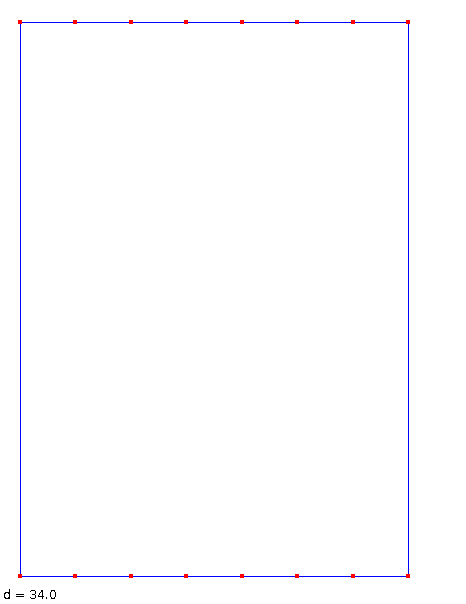
\includegraphics[scale=0.7]{images/16-32gen}\\
		Solution pour 16 villes, après 32 générations
	\end{center}
\end{figure}
\begin{figure}
	\begin{center}
		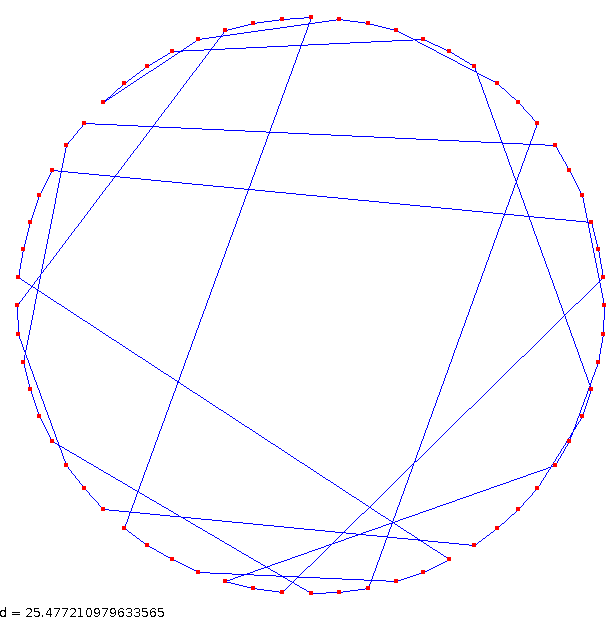
\includegraphics[scale=0.7]{images/64-1000gen}\\
		Solution pour 64 villes, après 1000 générations
	\end{center}
\end{figure}
\begin{figure}
	\begin{center}
		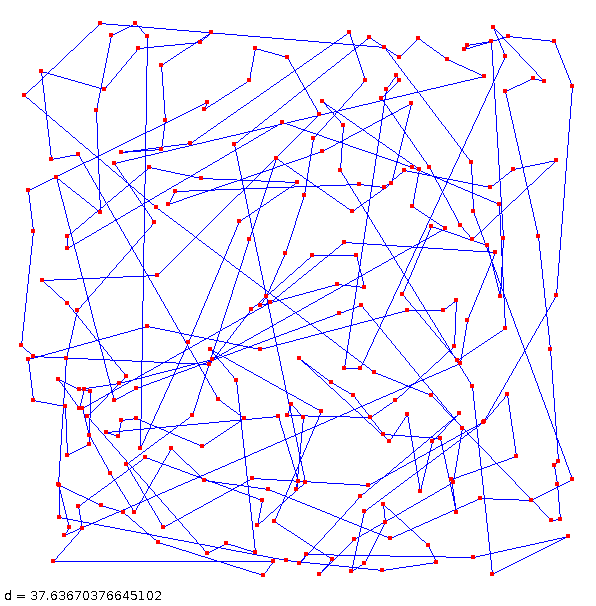
\includegraphics[scale=0.7]{images/250-1000gen}\\
		Solution pour 250 villes, après 1000 générations
	\end{center}
\end{figure}
\section{Conclusion}
On peut donc voir que l'algorithmie génétique est un outil très puissant qui permet de trouver rapidement des solutions convenables à des problèmes compliqués comme KS, TSP, etc. Mais généralement, une optimisation est nécessaire pour tirer pleinement profit de ce type de méthode. En effet, dans le cas de TSP, pour un nombre important de villes, l'algorithme a du mal à trouver une bonne solution lorsqu'il part de rien. Il nécessite alors des optimisations pour pouvoir converger vers une meilleure solution. 
\end{document}

